\section{Thermal Analysis of the PCB}

\subsection{Hypothesis}
The purpose of the thermal analysis is to validate that the Polyimide
PCB and the components can operate under the space conditions. The
operational temperature of Polyimide minimum is -240°C and the maximum
is 260°C. If the components are within the operational temperature
range, then it is validated to be operational under dynamic heat
conditions, however if it exceeds it, then the PCB material, and the PCB
design with the component locations must be altered and reworked. It is
expected that the photodiodes area of the PCB to have the most thermal
activity, with the lowest thermal activity occurring to the resisters.

\subsection{Thermal Analysis Parameters}
After a PCB CAD model is designed and material selection is completed,
the thermal analysis for the PCB can now be conducted. The PCB CAD model
was imported into ANSYS workbench using steady-state thermal analysis
and a mesh was applied generated to the model to influences the accuracy
and convergence of the simulation. Each of the components have their
respective materials applied to the model, such as the photodiodes with
silicon and aluminium, connectors being made of copper, nickel, zinc,
amplifiers and resisters made from aluminium, and the PCB being made of
polyimide. Then a convection of 22°C was applied to the side of the PCB
to simulate the transfer of heat of the PCB from the shuttlecraft it is
housed in, assumingly room temperature of the spacecraft is the same as
on Earth, it would be 22°C. Each of the components have their respective
temperatures when operating, this can be seen in Figure~\ref{fig:PCBparameters}Finally, two tests will be conducted using
200°C and -200°C of radiation applied to the entire PCB model to
simulate when the PCB is facing to the sun, and when the PCB is in the
shadows of celestial bodies respectively.

\begin{figure}[htbp]
    \centering
    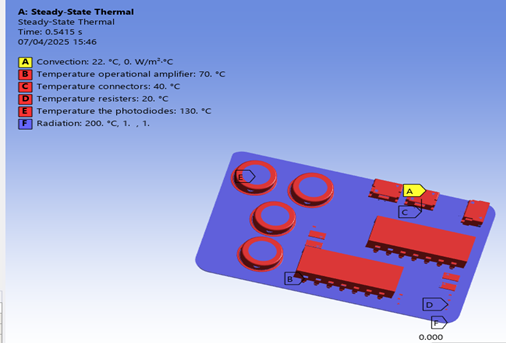
\includegraphics[width=0.8\textwidth]{chapters/methodology/ThermalAnalysis/Fig1parameters.png}
    \caption{PCB model with Parameters applied}
    \label{fig:PCBparameters}
\end{figure}
%%%%%%%%%%%%%%%%%%%%%%%%%%%%%%%%%%%%%%%%%%%%%%%%%%%%%%%%%%%

\section{Thermal results}

\subsection{Finite Analysis Evaluation 1 - Under 200°C in space}

\begin{figure}[htbp]
    \centering
    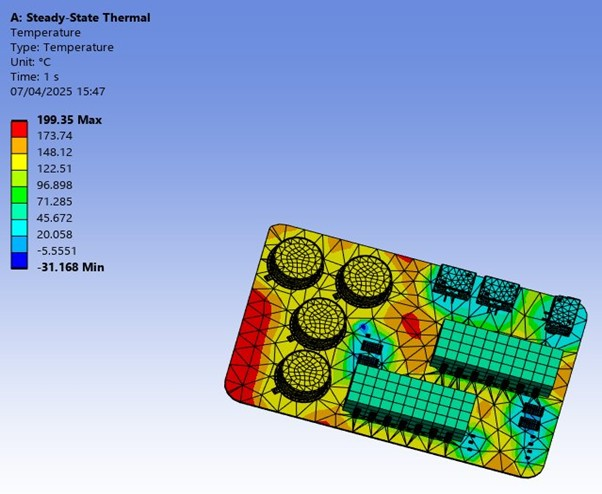
\includegraphics[width=0.95\textwidth]{chapters/methodology/ThermalAnalysis/Fig2under200C.jpg}
    \caption{Results under 200°C radiation}
    \label{fig:results_200C}
\end{figure}

The results for the PCB when facing towards the sun
depicts the most heat being towards outside of the photodiodes area and
the cooler parts are around the other components. As the figure~\ref{fig:results_200c}
shows the maximum temperature experienced is 199.35°C and the minimum
temperature is -31.168°C, this shows that the PCB can be operable when
facing towards the Sun.




\subsubsection{Finite Analysis Evaluation 2 (Under -200C in Space)}

The results for the PCB, when it is in the shadows of a celestial body, depicts the most heat coming from the photodiodes themselves which is to be expected as it creates the most heat in the PCB components followed by the amplifiers then connectors. As Figure~\ref{fig:results_minus_200C}  shows, the maximum temperature experienced is 136C and the minimum temperature is -173.83°C, this shows that the PCB can be operable when in the shadow of a celestial body.

\begin{figure}[htbp]
    \centering
    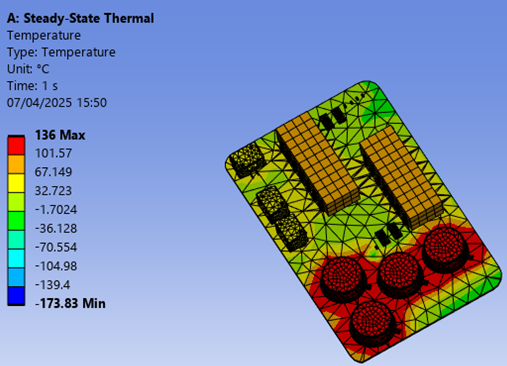
\includegraphics[width=0.8\textwidth]{chapters/methodology/ThermalAnalysis/Fig3underneg200c.png}
    \caption{Results under -200°C radiation}
    \label{fig:results_minus_200C}
\end{figure}

\subsection{Results Evaluation}

The results shown for both under +200°C and -200°C radiation shows that
the PCB is operable under the harsh thermal conditions in space. That
validates the design of the PCB and their component placements, and the
material selection. The polyimide having about a clearance when facing
the sun at 60°C and when in the shadows of a celestial object at -66°C
shows that it would not be on the brink of melting or freezing during
operation. The next step would be analysis the stresses and forces at
work in space, unfortunately, a mechanical analysis of the stress cannot
be conducted because it requires further work with the complete work of
the entirety of the CubeSat chassis and all the power source such as the
solar panels.
